\documentclass[../../main.tex]{subfiles}
\begin{document}

\subsection*{8.6}
Nei due circuiti in figura i raggi delle semicirconferenze sono $a=10\ cm$ e $b=15\ cm$.
\\Se la corrente vale $i = 20\ A$ calcolare per entrambi il campo magnetico $\vec{B_0}$ nel centro O delle semicirconferenze e il momento magnetico $\vec{m}$.
\\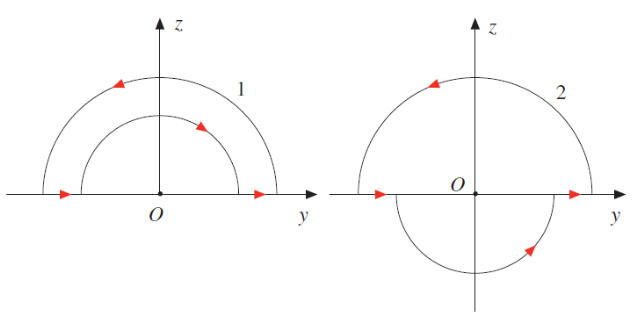
\includegraphics[scale=0.3]{e_8_6.png}
\subsubsection*{Formule utilizzate}
\subsubsection*{Soluzione punto a}
Il campo magnetico in O generato da ogni semicerchio si trova dimezzando l'espressione del camo di una spira circolare al centro della spira oppure applicando direttamente la prima legge elementare di Laplace:
\\$\vec{B_0} = \frac{\mu_0 i}{4b}\vec{u_x}-\frac{\mu_0 i}{4a}\vec{u_x}$
\\essendo che i due tratti rettilinei danno contributo nullo $(d\vec{s} \parallel \vec{u_r})$. Numericamente:
\\$B_0 = \frac{1.26 * 10^{-6} * 20}{4}\left(\frac{1}{0.15}-\frac{1}{0.1}\right) = -2.1 * 10^{-5}\ T$
\\$\vec{m} = i\frac{\pi}{2}\left(b^2 - a^2\right)\vec{u_x}=0.39\vec{u_x}\ Am^2$
\\Procedendo come prima
\\$\vec{B_0} = \frac{\mu_0 i}{4b}\vec{u_x}+\frac{\mu_0 i}{4a}\vec{u_x}$
\\essendo che i due tratti rettilinei
\\$B_0 = \frac{1.26 * 10^{-6} * 20}{4}\left(\frac{1}{0.15}+\frac{1}{0.1}\right) = 10.5* 10^{-5}\ T$
\\$\vec{m} = i\frac{\pi}{2}\left(b^2 + a^2\right)\vec{u_x}=1.02\vec{u_x}\ Am^2$

\subsubsection*{Soluzione punto b}
\newpage

\end{document}